\documentclass[12pt,letterpaper]{article}
\usepackage[utf8]{inputenc}
\usepackage[spanish]{babel}
\usepackage{graphicx}
\usepackage[left=2cm,right=2cm,top=2cm,bottom=2cm]{geometry}
\usepackage{graphicx} % figuras
% \usepackage{subfigure} % subfiguras
\usepackage{float} % para usar [H]
\usepackage{amsmath}
%\usepackage{txfonts}
\usepackage{stackrel} 
\usepackage{multirow}
\usepackage{enumerate} % enumerados
\renewcommand{\labelitemi}{$-$}
\renewcommand{\labelitemii}{$\cdot$}


% \author{}
% \title{Caratula}
\begin{document}

% Fancy Header and Footer
% \usepackage{fancyhdr}
% \pagestyle{fancy}
% \cfoot{}
% \rfoot{\thepage}
%

% \usepackage[hidelinks]{hyperref} % CREA HYPERVINCULOS EN INDICE

% \author{}
\title{Caratula}

\begin{titlepage}
\begin{center}
\large{UNIVERSIDAD PRIVADA DE TACNA}\\
\vspace*{-0.025in}
\begin{figure}[htb]
\begin{center}

\includegraphics[width=8cm]{./Imagenes/logo}
\end{center}
\end{figure}
\vspace*{0.15in}
INGENIERIA DE SISTEMAS  \\

\vspace*{0.5in}
\begin{large}
TITULO:\\
\end{large}

\vspace*{0.1in}
\begin{Large}
\textbf{Informe 07 Cuestionario de  Base de datos Oracle} \\
\end{Large}

\vspace*{0.3in}
\begin{Large}
\textbf{CURSO:} \\
\end{Large}

\vspace*{0.1in}
\begin{large}
BASE DE DATOS II\\
\end{large}

\vspace*{0.3in}
\begin{Large}
\textbf{DOCENTE(ING):} \\
\end{Large}

\vspace*{0.1in}
\begin{large}
 Patrick Cuadros Quiroga\\
\end{large}

\vspace*{0.2in}
\vspace*{0.1in}
\begin{large}
Alumno: \\
\begin{flushleft}
Jhon Peter Aguilar Atencio\hfill 	(2015053222) \\
Guimer Senon Coaquira Coaquira\hfill 	(2015053226) \\
\end{flushleft}
\end{large}
\end{center}

\end{titlepage}


\tableofcontents % INDICE
\thispagestyle{empty} % INDICE SIN NUMERO
\newpage
\setcounter{page}{1} % REINICIAR CONTADOR DE PAGINAS DESPUES DEL INDICE


\begin{Large}
\begin{center}
\textbf{Trabajo Encargado} \\
\end{center}
\end{Large}

\section{Objetivos} 


\begin{itemize}

 Crear un esquema de base de datos.
\\\\
 Crear objetos de tipo tabla dentro de la base de datos.\\

\end{itemize} 

\section{Requerimientos} 

\begin{itemize}
 Conocimientos\\\\
Para el desarrollo de esta práctica se requerirá de los siguientes conocimientos básicos:\\
- Conocimientos básicos de comandos Linux a nivel de consola o terminal de texto.\\
- Conocimientos básicos de redes locales.\\
 Software\\\\
Asimismo se necesita los siguientes aplicativos:\\
- Máquina Virtual conteniendo la versión 11g de Oracle Database instalada sobre un sistema operativo Oracle
Linux Server.\\
- Herramienta de desarrollo SQL Developer\\



\end{itemize} 

\section{Pasos a seguir}
\begin{itemize}
    
    
\end{itemize}

\begin{itemize}
	\begin{center}
	    Ejercicio 1
	\end{center}
	

	    Desarrollar el script de creación de TableSpace(s) y archivos para la base de datos de su proyecto.\\\\
	    
	    
	    
		\begin{center}
		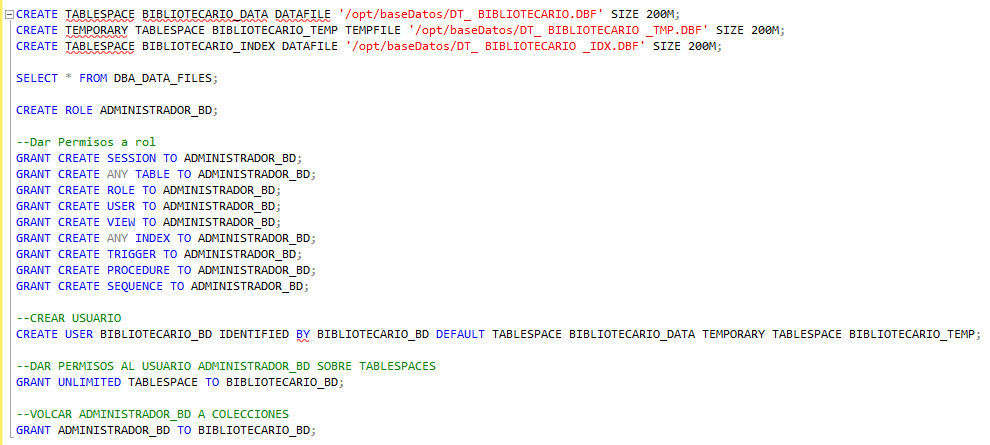
\includegraphics[width=15cm]{./Imagenes/imagen1} 
		\end{center}
	

	\end{itemize} 
	

	\begin{itemize}
	\begin{center}
	    Ejercicio 2
	\end{center}
	

	    Desarrollar el script de creación de objetos (entidades, atributos, llaves y restricciones). \\\\
		\begin{center}
		\includegraphics[width=15cm]{./Imagenes/imagen2} 
		\end{center}
	

	\end{itemize} 
	

  
  
  


\include{Secciones/bibliografia}


\end{document}
